\steppingstone{Mirrors}
\label{stone:mirrors}

A mirror is one of the simplest objects in geometry. It changes a construction without stretching it, shrinking it, or breaking it apart. Distances remain the same. Angles remain the same. Only one thing changes. Every point appears on the opposite side of the mirror at exactly the same distance from it.

If PhiBase really belongs to geometry, it should be able to follow that journey exactly.

Rather than beginning with a formula, let us begin with a construction. Choose one point whose six-beam address is already known. Translate it into Cartesian coordinates. Reflect it across one of the six working mirrors. Finally, translate the reflected point back into a six-beam description. Figure~\ref{fig:reflection-example} follows that complete journey.

\begin{figure}[htbp]
\centering
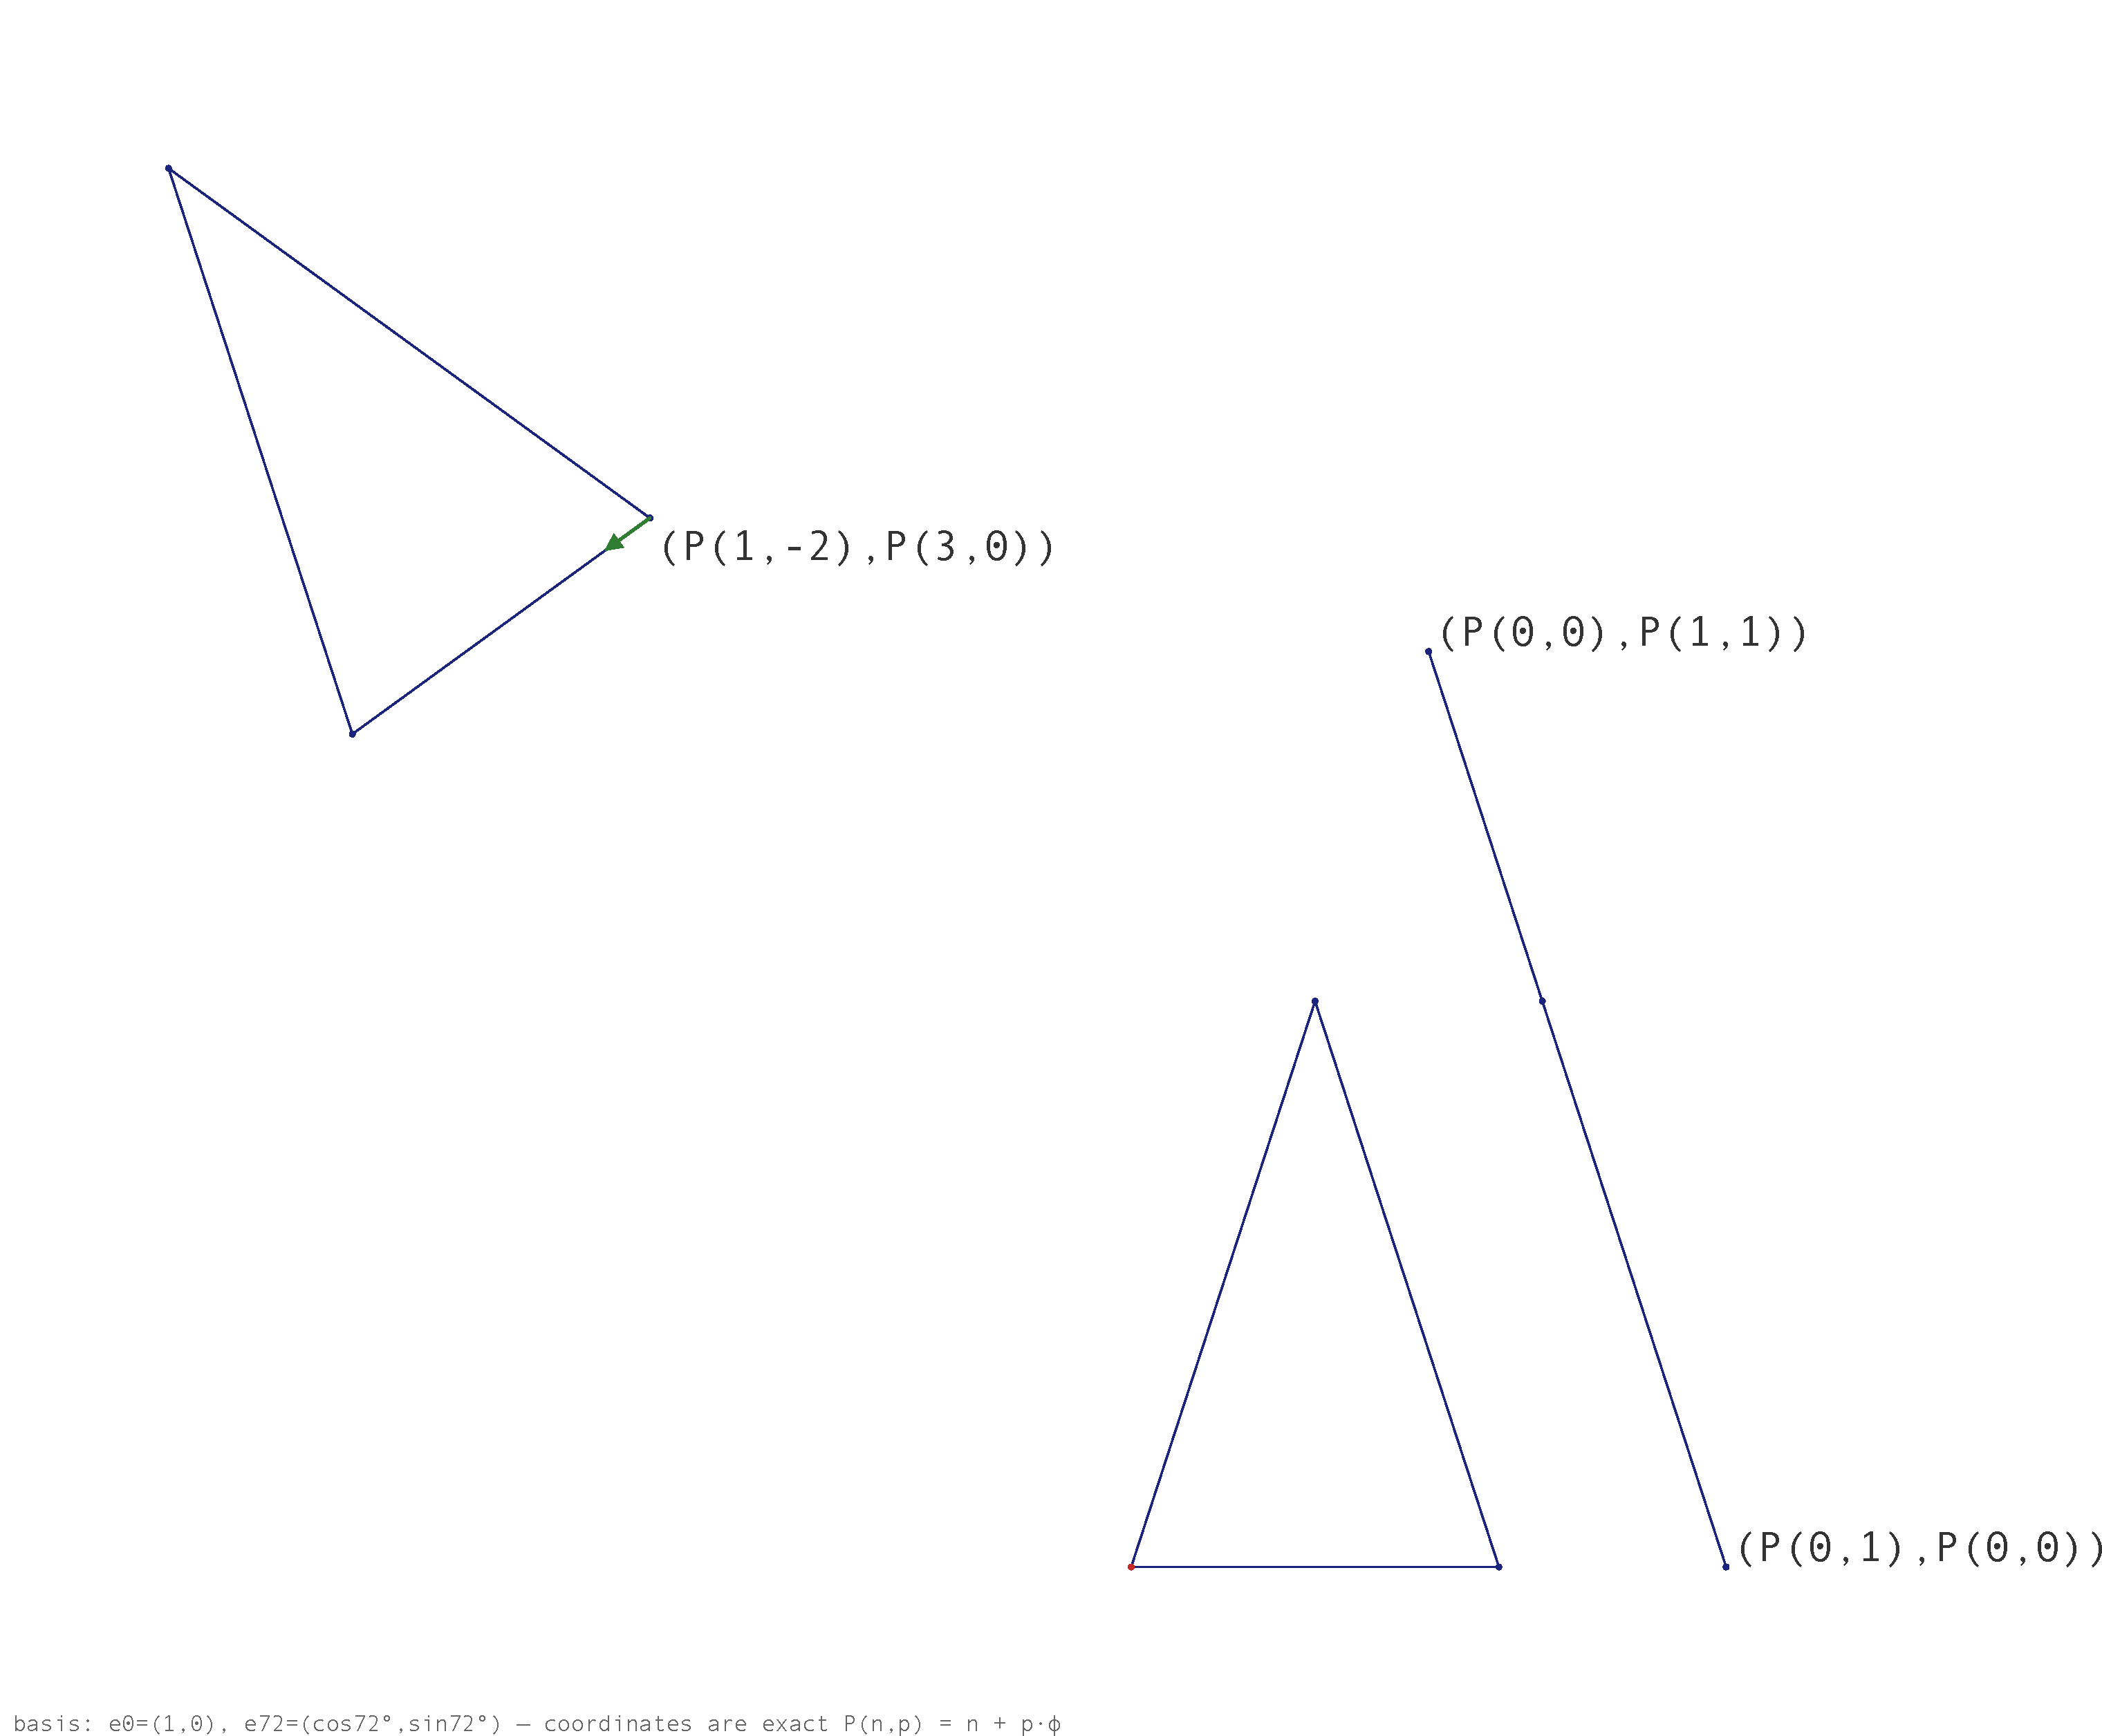
\includegraphics[width=.95\textwidth]{figures/turtle/reflection-example.pdf}
\caption{One complete reflection. Every stage is exact. The construction begins with a lattice point, reflects it across a working mirror, and returns to a six-beam description.}
\label{fig:reflection-example}
\end{figure}

Before reading further, work through the figure yourself. The arithmetic is deliberately uncomplicated. Each step follows from ideas that have already appeared in earlier stepping stones.

Now look at the reflected coordinates.

Nothing has been rounded.

Nothing has been approximated.

The reflected point is still exact.

Yet something new has appeared.

Every coordinate carries the same denominator,

\[
5.
\]

Repeat the construction for another point.

The same denominator appears again.

Reflect a third point.

Once more the denominator is five.

By now it is difficult to believe that this is a coincidence.

The geometry is trying to tell us something.

The answer is hidden inside the mirror itself.

Every mirror has a direction pointing straight away from its surface. Mathematicians call that direction the normal. For each of the six working mirrors, the normal has the PhiBase length

\[
\varphi+2.
\]

Yesterday we learned how to find the conjugate of a PhiBase quantity. Let us do exactly the same thing here. Multiply

\[
\varphi+2
\]

by its conjugate. The result is simply

\[
5.
\]

The denominator did not appear because of the reflection formula. It was already present in the geometry of the mirror. The arithmetic merely uncovered it.

That observation changes the way we should think about the reflected point. It has not left PhiBase. It has simply entered a slightly larger landscape,

\[
\frac{1}{5}\mathbb{Z}[\varphi].
\]

Some reflected points return immediately to the original six-beam lattice. Others remain between ordinary lattice points. Both are exact. The difference is not accuracy but location.

The mirror has revealed structure that was already present but had remained hidden.

That has happened before.

The Fibonacci Spine was already there before we noticed it. The conjugate was already there before we searched for it. The denominator of five belongs to the same family of discoveries. The geometry asked the question. The arithmetic answered it.

\section*{Builder's Notebook}

Repeat the reflection shown in Figure~\ref{fig:reflection-example} for a second point. Then reflect the result across the same mirror. The second reflection should return you exactly to your starting point.

A mirror always undoes itself.

The arithmetic should do the same.

\section*{Looking Ahead}

We have now built an exact arithmetic for lengths, constructions, space, and symmetry. One final question remains.

Can a machine follow these same constructions as faithfully as we can?
